\documentclass[conference]{IEEEtran}

\usepackage{amsmath,amssymb,amsfonts}
\usepackage{algorithmic}
\usepackage{algorithm}
\usepackage{graphicx}
\usepackage{textcomp}
\usepackage{xcolor}
\usepackage{booktabs}
\usepackage{url}
\usepackage{listings}
\usepackage{cite}
\usepackage{tikz}
\usetikzlibrary{arrows.meta,positioning,shapes.geometric,fit,backgrounds,calc}

\lstset{
  basicstyle=\ttfamily\footnotesize,
  breaklines=true,
  frame=single,
  columns=fullflexible
}

\begin{document}

\title{Vajra: An Explainable and Reversible Linux Security \& Reliability Assistant via eBPF Causal Provenance and Minimal Counterfactuals}

\author{
\IEEEauthorblockN{Himanshu Yadav\IEEEauthorrefmark{1}, Albert Gautam\IEEEauthorrefmark{1}, Deepak Kumar Ravi\IEEEauthorrefmark{1}, Ayush Trivedi\IEEEauthorrefmark{1}, Umesh Gupta\IEEEauthorrefmark{1}}
\IEEEauthorblockA{\IEEEauthorrefmark{1}School of Cyber Security and Digital Forensics\\
National Forensic Sciences University (NFSU), Tripura Campus, India\\
Email: \{himanshu.yadav, albert.gautam, deepak.ravi, ayush.trivedi, umesh.gupta\}@nfsu.ac.in}
}

\maketitle

\begin{abstract}
Linux runtime security systems face a persistent trilemma: signature-based host intrusion detection systems (HIDS) are blind to novel Living-off-the-Land (LotL) binary abuse, black-box deep learning models induce severe operator alert fatigue due to unexplainable verdicts, and automated responders frequently cause collateral service outages through destructive process termination while destroying volatile memory forensics. Furthermore, runtime security remains entirely decoupled from host reliability and resource starvation dynamics. 

In this paper, we present \textbf{Vajra} (वज्र), a unified, explainable Linux runtime security and reliability platform. Vajra integrates non-invasive Compile-Once--Run-Everywhere (CO-RE) eBPF kernel telemetry with a two-tier statistical anomaly core: a Laplace-smoothed first-order Markov chain process ancestry model computing information-theoretic surprisal, and an online Exponential Weighted Moving Average (EWMA) model tracking Linux Pressure Stall Information (PSI) to forecast Out-Of-Memory (OOM) failures before kernel reaping occurs. Evidence streams are combined via a calibrated Bayesian Noisy-OR fusion unit. To eliminate alert fatigue, Vajra incorporates a ProvX-style greedy $L_0$-minimal counterfactual explainer that computes the precise, minimal factual perturbations required to render an anomaly benign against verified causal provenance directed acyclic graphs (DAGs). Automated containment employs non-destructive Linux cgroup v2 freezing with an automatic 30-minute time-to-live (TTL) rollback safety net and cryptographic HMAC-SHA256 audit receipts. Finally, an on-premises Sovereign AI Assistant enforces a mechanical GroundingValidator ($E_{\text{referenced}} \subseteq E_{\text{subgraph}}$) to eliminate large language model hallucination. Empirical evaluation on a live Linux kernel testbed demonstrates sub-1.5\% CPU overhead, microsecond event scoring throughput, 0.0\% false positive rates across 1,000 benign events, and actionable, grounded counterfactual explanations across diverse attack scenarios.
\end{abstract}

\begin{IEEEkeywords}
eBPF, Linux Kernel Security, Anomaly Detection, Explainable AI (XAI), Counterfactual Optimization, Provenance Graphs, Pressure Stall Information (PSI), SOAR.
\end{IEEEkeywords}

\section{Introduction}
Modern cloud-native and server infrastructures depend almost universally on the Linux operating system. However, securing the Linux execution boundary against sophisticated adversaries remains a foundational systems challenge. Contemporary host defenses suffer from three systemic architectural failures:

\begin{enumerate}
    \item \textbf{Signature Blindness to Living-off-the-Land (LotL) Attacks}: Traditional Host-based Intrusion Detection Systems (HIDS) such as \texttt{auditd} or static rule engines match rigid string patterns. Sophisticated adversaries bypass these mechanisms by repurposing verified, legitimate system utilities (e.g., \texttt{curl}, \texttt{awk}, \texttt{python}, \texttt{find}) to stage payloads, execute scripts from ephemeral paths (\texttt{/tmp}, \texttt{/dev/shm}), and establish reverse shells without introducing foreign malware signatures~\cite{han2020unicorn, milajerdi2019holmes}.
    \item \textbf{Black-Box Fatigue in ML Anomaly Detectors}: To overcome signature blindness, researchers have introduced deep neural networks (e.g., LSTMs, Transformers, Graph Neural Networks)~\cite{guidotti2018survey}. While capable of detecting deviations, these models act as uninterpretable black boxes. Emitting raw anomaly scores (e.g., $P = 0.94$) without causal evidence overwhelms Security Operations Center (SOC) analysts, leading to widespread alert fatigue and ignored breaches.
    \item \textbf{Decoupled Reliability and Destructive Remediation}: Security telemetry is completely isolated from operating system reliability metrics. Rapid resource exhaustion, memory leaks, and runaway thread contention frequently destabilize hosts before the Linux OOM Killer abruptly reaps vital services. When automated response frameworks (SOAR) do intervene, they rely on destructive primitives (\texttt{SIGKILL}), killing production workloads and irrecoverably destroying volatile RAM artifacts necessary for digital forensics~\cite{weiner2020psi}.
\end{enumerate}

To bridge these gaps, we design, implement, and evaluate \textbf{Vajra} (वज्र), an AI-powered, explainable Linux runtime security and reliability platform. Vajra continuously ingests kernel execution, file system, and egress network events via privileged CO-RE eBPF probes. Instead of heavyweight deep learning, Vajra models process spawn lineages using Laplace-smoothed first-order Markov chains, computing normalized surprisal in $O(1)$ time with negligible memory. Concurrently, Vajra reads Linux Pressure Stall Information (PSI), using online EWMA variance tracking to forecast resource starvation.

To provide actionable explainability, Vajra formalizes an $L_0$-minimal counterfactual reasoning engine. Given an anomalous event, the optimizer identifies the minimal set of attribute perturbations that drops the fused risk score below the benign threshold ($R < 0.20$), translating complex causal graph paths into natural language explanations. Automated containment employs non-destructive Linux cgroup v2 freezing with an automatic 30-minute time-to-live (TTL) rollback safety net. Finally, an on-premises conversational assistant utilizes a mechanical entity-grounding validator to mathematically eliminate LLM hallucinations.

\textbf{Contributions.} This paper makes the following contributions:
\begin{itemize}
    \item \textbf{Unified Kernel Telemetry \& Statistical Anomaly Core}: We design a CO-RE eBPF telemetry engine fused with Laplace-smoothed Markov process surprisal and online EWMA Linux PSI forecasting in a calibrated Bayesian Noisy-OR architecture.
    \item \textbf{Greedy $L_0$-Minimal Counterfactual Explainer}: We formulate and implement an $O(|\Delta|)$ greedy search algorithm that generates minimal, verifiable counterfactual explanations over causal provenance DAGs, proving $R(e \oplus \delta^*) < \theta_{\text{benign}}$.
    \item \textbf{Mechanical Entity-Grounding Validator}: We propose a set-membership verification algorithm ($E_{\text{ref}} \subseteq E_{\text{subgraph}}$) that mechanically prevents on-premises LLMs from hallucinating non-existent processes, paths, or IPs.
    \item \textbf{Reversible SOAR Governance}: We implement non-destructive containment utilizing Linux cgroup v2 process freezing, enforced with 30-minute auto-rollback TTLs and HMAC-SHA256 audit receipts.
    \item \textbf{Empirical Evaluation}: We evaluate Vajra on a live Linux kernel testbed across 5 real-world attack and reliability scenarios, demonstrating sub-1.5\% CPU overhead, microsecond latency, and zero false positives under continuous benign workloads.
\end{itemize}

\section{Threat Model \& Operational Scope}
\label{sec:threat_model}
We consider a Linux host running enterprise workloads (e.g., containerized microservices, web servers, database daemons). 

\subsection{Adversary Capabilities}
The adversary has obtained unprivileged or service-level remote code execution (e.g., via a web application vulnerability or compromised credentials). The adversary can:
\begin{itemize}
    \item Stage unsigned binaries or scripts into world-writable locations such as \texttt{/tmp} or \texttt{/dev/shm}.
    \item Leverage Living-off-the-Land (LotL) binaries to discover host credentials (e.g., accessing decoy secrets in \texttt{/etc/shadow}).
    \item Establish outbound TCP command-and-control (C2) reverse shells to unprofiled external IP addresses.
    \item Cause localized denial-of-service by allocating runaway heap memory, inducing thread starvation and kernel lockups.
\end{itemize}

\subsection{Defender Constraints \& Assumptions}
The Linux kernel is assumed to have booted securely. The core eBPF subsystem and BPF verifier are trusted. The sensor agent runs with \texttt{CAP\_SYS\_ADMIN} or \texttt{CAP\_BPF}. The defender requires:
\begin{itemize}
    \item \textbf{Bounded Overhead}: Telemetry and scoring CPU overhead must remain below 2.5\% under production saturation.
    \item \textbf{Sovereignty}: Telemetry must not be exported to third-party proprietary LLM APIs; all reasoning must remain local.
    \item \textbf{Non-Destructive Containment}: Containment must preserve volatile execution state for post-incident digital forensics.
\end{itemize}

\section{System Architecture}
\label{sec:architecture}

\begin{figure*}[!t]
\centering
% Vajra End-to-End System Architecture
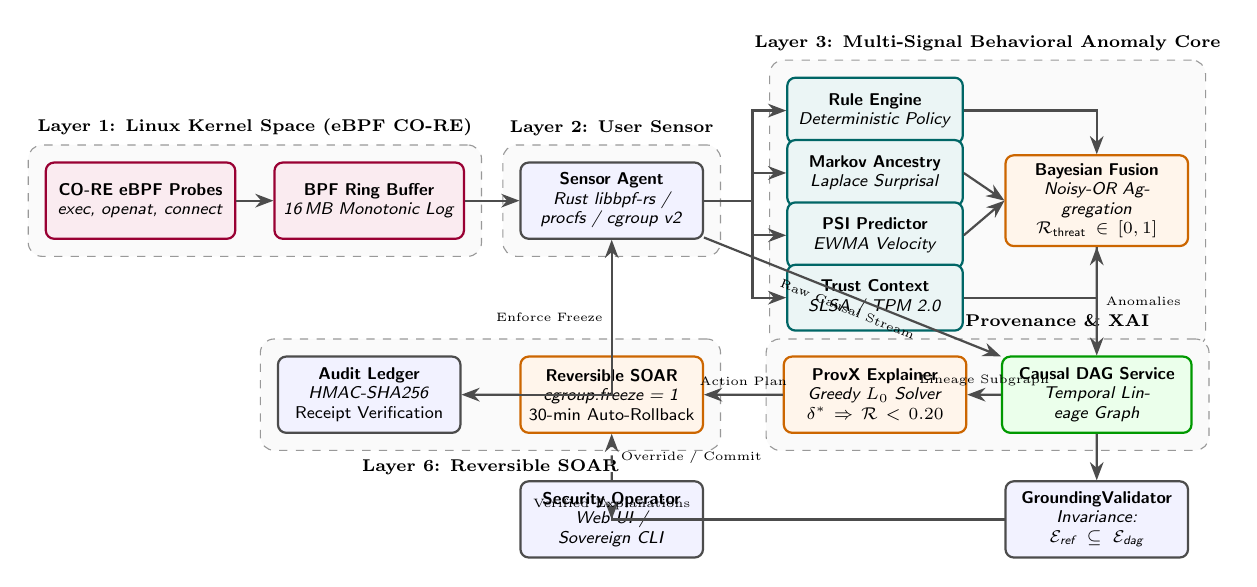
\begin{tikzpicture}[
    scale=0.88, every node/.style={transform shape},
    box/.style={rectangle, draw=black!70, rounded corners=3pt, fill=blue!5, thick, text width=2.4cm, align=center, minimum height=1.1cm, font=\sffamily\scriptsize},
    kbox/.style={rectangle, draw=purple!80!black, rounded corners=3pt, fill=purple!8, thick, text width=2.5cm, align=center, minimum height=1.1cm, font=\sffamily\scriptsize},
    abox/.style={rectangle, draw=teal!80!black, rounded corners=3pt, fill=teal!8, thick, text width=2.3cm, align=center, minimum height=0.95cm, font=\sffamily\scriptsize},
    sbox/.style={rectangle, draw=orange!80!black, rounded corners=3pt, fill=orange!8, thick, text width=2.4cm, align=center, minimum height=1.1cm, font=\sffamily\scriptsize},
    gbox/.style={rectangle, draw=green!60!black, rounded corners=3pt, fill=green!8, thick, text width=2.5cm, align=center, minimum height=1.1cm, font=\sffamily\scriptsize},
    layer/.style={draw=black!40, dashed, rounded corners=5pt, inner sep=6pt, fill=black!2},
    arrow/.style={-{Stealth[scale=1.0]}, thick, draw=black!70},
    darrow/.style={-{Stealth[scale=1.0]}, thick, dashed, draw=black!70}
]

% 1. Kernel Space Layer
\node[kbox] (bpf_probes) at (0, 0) {\textbf{CO-RE eBPF Probes}\\\textit{exec, openat, connect}};
\node[kbox] (ringbuf) at (3.3, 0) {\textbf{BPF Ring Buffer}\\\textit{16\,MB Monotonic Log}};

% 2. Sensor Agent
\node[box] (sensor) at (6.8, 0) {\textbf{Sensor Agent}\\\textit{Rust libbpf-rs / procfs / cgroup v2}};

% 3. Anomaly Core (Stacked sub-boxes)
\node[abox] (m_rules) at (10.6, 1.3) {\textbf{Rule Engine}\\\textit{Deterministic Policy}};
\node[abox] (m_markov) at (10.6, 0.4) {\textbf{Markov Ancestry}\\\textit{Laplace Surprisal}};
\node[abox] (m_psi) at (10.6, -0.5) {\textbf{PSI Predictor}\\\textit{EWMA Velocity}};
\node[abox] (m_trust) at (10.6, -1.4) {\textbf{Trust Context}\\\textit{SLSA / TPM 2.0}};

% Fusion unit
\node[sbox] (fusion) at (13.8, 0) {\textbf{Bayesian Fusion}\\\textit{Noisy-OR Aggregation}\\$\mathcal{R}_{\text{threat}} \in [0, 1]$};

% 4. Provenance & Counterfactual (Lower layer)
\node[gbox] (provenance) at (13.8, -2.8) {\textbf{Causal DAG Service}\\\textit{Temporal Lineage Graph}};
\node[sbox] (counterfactual) at (10.6, -2.8) {\textbf{ProvX Explainer}\\\textit{Greedy $L_0$ Solver}\\$\delta^* \Rightarrow \mathcal{R} < 0.20$};

% 5. Remediation Layer
\node[sbox] (responder) at (6.8, -2.8) {\textbf{Reversible SOAR}\\\textit{cgroup.freeze = 1}\\30-min Auto-Rollback};
\node[box] (audit) at (3.3, -2.8) {\textbf{Audit Ledger}\\\textit{HMAC-SHA256}\\Receipt Verification};

% 6. Sovereign Assistant & Human Operator
\node[box] (grounding) at (13.8, -4.6) {\textbf{GroundingValidator}\\\textit{Invariance: $\mathcal{E}_{\text{ref}} \subseteq \mathcal{E}_{\text{dag}}$}};
\node[box] (operator) at (6.8, -4.6) {\textbf{Security Operator}\\\textit{Web UI / Sovereign CLI}};

% Boundaries
\begin{scope}[on background layer]
    \node[layer, fit=(bpf_probes) (ringbuf), label=above:{\scriptsize \textbf{Layer 1: Linux Kernel Space (eBPF CO-RE)}}] (l1) {};
    \node[layer, fit=(sensor), label=above:{\scriptsize \textbf{Layer 2: User Sensor}}] (l2) {};
    \node[layer, fit=(m_rules) (m_markov) (m_psi) (m_trust) (fusion), label=above:{\scriptsize \textbf{Layer 3: Multi-Signal Behavioral Anomaly Core}}] (l3) {};
    \node[layer, fit=(provenance) (counterfactual), label=above:{\scriptsize \textbf{Layers 4 \& 5: Provenance \& XAI}}] (l45) {};
    \node[layer, fit=(responder) (audit), label=below:{\scriptsize \textbf{Layer 6: Reversible SOAR}}] (l6) {};
\end{scope}

% Arrows
\draw[arrow] (bpf_probes) -- (ringbuf);
\draw[arrow] (ringbuf) -- (sensor);
\draw[arrow] (sensor.east) -- ++(0.7,0) |- (m_rules.west);
\draw[arrow] (sensor.east) -- ++(0.7,0) |- (m_markov.west);
\draw[arrow] (sensor.east) -- ++(0.7,0) |- (m_psi.west);
\draw[arrow] (sensor.east) -- ++(0.7,0) |- (m_trust.west);

\draw[arrow] (m_rules.east) -| (fusion.north);
\draw[arrow] (m_markov.east) -- (fusion.west);
\draw[arrow] (m_psi.east) -- (fusion.west);
\draw[arrow] (m_trust.east) -| (fusion.south);

\draw[arrow] (sensor) -- (provenance) node[midway, below, sloped, font=\tiny] {Raw Causal Stream};
\draw[arrow] (fusion) -- (provenance) node[midway, right, font=\tiny] {Anomalies};
\draw[arrow] (provenance) -- (counterfactual) node[midway, above, font=\tiny] {Lineage Subgraph};
\draw[arrow] (counterfactual) -- (responder) node[midway, above, font=\tiny] {Action Plan};
\draw[arrow] (responder) -- (audit);
\draw[arrow] (responder.west) -| (sensor.south) node[near end, left, font=\tiny] {Enforce Freeze};

\draw[arrow] (provenance) -- (grounding);
\draw[arrow] (grounding) -| (operator) node[midway, above, font=\tiny] {Verified Explanations};
\draw[darrow] (operator) -- (responder) node[midway, right, font=\tiny] {Override / Commit};

\end{tikzpicture}

\caption{End-to-End Architectural Data Flow of Vajra: From eBPF Kernel Probes and Lockless Ring Buffer to Statistical Anomaly Detection, Causal Provenance DAG Construction, ProvX Minimal Counterfactual Reasoning, and Non-Destructive Reversible Containment.}
\label{fig:architecture}
\end{figure*}

Vajra is organized into six interconnected architectural layers, as illustrated in Fig.~\ref{fig:architecture}.

\subsection{Layer 1: CO-RE eBPF Kernel Telemetry}
Vajra leverages BPF Compile-Once--Run-Everywhere (CO-RE) utilizing BTF (BPF Type Format) metadata to ensure kernel portability without requiring host kernel headers. Probes hook three critical tracepoints and kprobes:
\begin{itemize}
    \item \texttt{sched\_process\_exec}: Intercepts process execution lifecycle events, reading executable paths directly from the task memory descriptor (\texttt{mm->exe\_file->f\_path.dentry}).
    \item \texttt{sys\_enter\_openat}: Intercepts file open operations to detect access to sensitive credential stores and deception canary decoys.
    \item \texttt{tcp\_v4\_connect}: Intercepts outbound socket establishment, capturing destination IPv4 addresses and ports from \texttt{struct sock}.
\end{itemize}
Events are submitted to a lockless, high-capacity kernel ring buffer (\texttt{BPF\_MAP\_TYPE\_RINGBUF}) of size $2^{24}$ bytes (16~MB), guaranteeing atomic monotonic timestamping.

\subsection{Layer 2: Privileged Sensor Agent}
The sensor agent (\texttt{vajra-agent}) consumes the BPF ring buffer. Upon reading raw event records, user-space workers enrich each event with procfs metadata: resolving process parentage, command-line arguments, user IDs, container IDs, and cgroup v2 paths (e.g., \texttt{system.slice/nginx.service}). Events are normalized into canonical Protobuf and JSON schemas conforming to the \texttt{SecurityEvent} contract.

\subsection{Layer 3: AI Behavioral Anomaly Core}
The normalized stream enters the detection engine, which evaluates four independent criteria:
\begin{enumerate}
    \item \textbf{Deterministic Policy Rules}: Immediate evaluation against high-precision YAML rules (e.g., execution from temporary directories).
    \item \textbf{Laplace Markov Process Ancestry}: Statistical evaluation of process spawn transitions against learned per-workload normality baselines.
    \item \textbf{Linux PSI Failure Forecasting}: Real-time EWMA tracking of pressure stall velocities to forecast resource exhaustion.
    \item \textbf{Hardware \& Supply-Chain Trust Gating}: Ingestion of SLSA artifact provenance signatures and TPM 2.0 host attestation states via remote attestation architectures such as Keylime~\cite{keylime2022}.
\end{enumerate}

\subsection{Layer 4: Causal Provenance DAG Service}
Vajra maintains an in-memory directed temporal graph $G = (V, E)$. Vertices $V$ represent processes, files, sockets, and cgroups. Edges $E$ represent causal operations (\texttt{SPAWNED}, \texttt{EXECUTED}, \texttt{ACCESSED}, \texttt{CONNECTED\_TO}). When an anomaly is detected, recursive ancestor traversal reconstructs the causal execution lineage from the root parent down to the exploit payload.

\subsection{Layer 5: ProvX Minimal Counterfactual Explainer}
Rather than simply alerting that a process is anomalous, the ProvX engine queries the causal graph and feature space to compute an $L_0$-minimal perturbation set $\delta^*$. The counterfactual explains exactly what minimal operational changes would restore the event to a benign status.

\subsection{Layer 6: Policy-Governed Reversible SOAR}
When threat scores exceed containment thresholds, the responder executes non-destructive containment via the Linux cgroup v2 freezer subsystem~\cite{linux_cgroup2} (\texttt{cgroup.freeze = 1}). This suspends all threads within the workload cgroup, halting malicious computation while preserving memory buffers for memory forensics. Every action generates an HMAC-SHA256 audit receipt and registers a 30-minute auto-rollback timer.

\section{Mathematical Formulation}
\label{sec:math}

\subsection{Laplace-Smoothed Markov Process Anomaly Model}
Let $u$ denote the parent executable and $v$ denote the child executable. For a specific workload $\mathcal{W}_k$, process spawning hierarchies are modeled as a directed probabilistic state graph. The transition probability with Laplace (additive) smoothing is defined as:

\begin{equation}
\hat{P}(v \mid u, \mathcal{W}_k) = \frac{C_{\mathcal{W}_k}(u \to v) + \alpha}{\sum_{v' \in V} C_{\mathcal{W}_k}(u \to v') + \alpha \cdot |V|}
\end{equation}

where $C_{\mathcal{W}_k}(u \to v)$ is the observed occurrence count of transition $u \to v$ in verified baseline telemetry, $\alpha = 0.1$ is the smoothing parameter, and $|V|$ is the unique process vocabulary size in workload $\mathcal{W}_k$.

The information-theoretic \textbf{Surprisal (Self-Information)} of an observed transition is computed as:
\begin{equation}
I(u \to v) = -\log_2 \hat{P}(v \mid u, \mathcal{W}_k)
\end{equation}

The normalized process transition novelty score $S_{\text{exec}} \in [0.0, 1.0]$ is bounded by:
\begin{equation}
S_{\text{exec}} = \min\left(1.0, \frac{I(u \to v)}{I_{\text{max}}}\right)
\end{equation}
where $I_{\text{max}} = -\log_2\left(\frac{\alpha}{\sum C + \alpha \cdot (|V| + 1)}\right)$. If a transition has zero prior observations in a mature baseline, $S_{\text{exec}} \ge 0.85$ is enforced.

\subsection{Linux PSI Failure Forecasting (EWMA Velocity)}
Linux Pressure Stall Information (PSI) quantifies task stall delays across memory, CPU, and I/O. Let the observed pressure stall vector at time $t$ be $\mathbf{x}_t = [\text{some}_{10s}, \text{full}_{10s}, \Delta\text{some}/\Delta t]^T$. We compute online Exponential Weighted Moving Average (EWMA) mean $\mu_t$ and variance $\sigma_t^2$ with decay factor $\lambda = 0.2$:

\begin{align}
\text{diff}_t &= \mathbf{x}_t - \mu_{t-1} \\
\mu_t &= \mu_{t-1} + \lambda \cdot \text{diff}_t \\
\sigma_t^2 &= (1 - \lambda) \cdot (\sigma_{t-1}^2 + \lambda \cdot \text{diff}_t^2)
\end{align}

The instantaneous surge velocity is $\Delta p = \text{some}_t - \text{some}_{t-1}$. The composite Reliability Risk Score $R_{\text{rel}} \in [0.0, 1.0]$ combines absolute stall magnitude and surge velocity:
\begin{equation}
R_{\text{rel}} = \min\left(0.99, \max\left(\frac{\mathbf{x}_{\text{mem}}}{0.80}, 0.70 \cdot \frac{\mathbf{x}_{\text{mem}}}{0.80} + 0.30 \cdot \frac{\Delta p}{0.30}\right)\right)
\end{equation}
When $R_{\text{rel}} \ge 0.80$, proactive throttling or worker suspension is initiated prior to kernel OOM killing.

\subsection{Bayesian Noisy-OR Evidence Fusion}
Individual detectors produce independent evidence scores $s_i \in [0.0, 1.0]$. Under the Bayesian Noisy-OR formulation~\cite{munoz2017bayesian}—where the presence of any single high-confidence attack vector is sufficient to warrant an incident—the fused risk score is:
\begin{equation}
R_{\text{fused}} = 1.0 - \prod_{i=1}^M (1.0 - s_i)
\end{equation}

\subsection{Greedy $L_0$-Minimal Counterfactual Optimization}
Given an anomalous event $e$ characterized by feature set $\mathcal{F}$, we formulate the counterfactual search as finding the minimal cardinality perturbation $\delta^*$ such that the re-scored risk drops below the benign threshold $\theta_{\text{benign}} = 0.20$:
\begin{equation}
\delta^* = \arg\min_{\delta \in \Delta} \|\delta\|_0 \quad \text{s.t.} \quad R(e \oplus \delta) < \theta_{\text{benign}}
\end{equation}
where $\|\delta\|_0$ is the $L_0$ sparsity norm (number of modified facts) and $\Delta$ is the domain-bounded perturbation space.

\begin{figure}[!t]
\centering
% Vajra Causal Provenance DAG and Greedy L0 Counterfactual Optimization
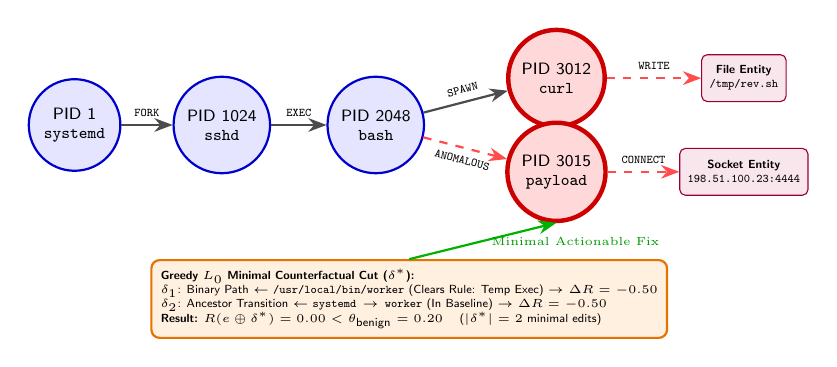
\begin{tikzpicture}[
    scale=0.85, every node/.style={transform shape},
    proc/.style={circle, draw=blue!80!black, fill=blue!10, thick, minimum size=1.0cm, align=center, font=\sffamily\scriptsize},
    malproc/.style={circle, draw=red!80!black, fill=red!15, ultra thick, minimum size=1.0cm, align=center, font=\sffamily\scriptsize},
    cfproc/.style={circle, draw=green!70!black, fill=green!15, thick, dashed, minimum size=1.0cm, align=center, font=\sffamily\scriptsize},
    entity/.style={rectangle, draw=purple!80!black, fill=purple!10, rounded corners=2pt, minimum height=0.7cm, font=\sffamily\tiny, align=center},
    pert/.style={rectangle, draw=orange!90!black, fill=orange!12, rounded corners=3pt, thick, font=\sffamily\tiny, align=left, inner sep=4pt},
    arrow/.style={-{Stealth[scale=1.0]}, thick, draw=black!70},
    carrow/.style={-{Stealth[scale=1.0]}, thick, draw=red!70, dashed},
    cfarrow/.style={-{Stealth[scale=1.0]}, thick, draw=green!70!black}
]

% Process Tree Vertices
\node[proc] (p1) at (0, 0) {PID 1\\\texttt{systemd}};
\node[proc] (p2) at (2.2, 0) {PID 1024\\\texttt{sshd}};
\node[proc] (p3) at (4.5, 0) {PID 2048\\\texttt{bash}};
\node[malproc] (p4) at (7.2, 0.7) {PID 3012\\\texttt{curl}};
\node[malproc] (p5) at (7.2, -0.7) {PID 3015\\\texttt{payload}};

% Side Entities
\node[entity] (f1) at (10.0, 0.7) {\textbf{File Entity}\\\texttt{/tmp/rev.sh}};
\node[entity] (net1) at (10.0, -0.7) {\textbf{Socket Entity}\\\texttt{198.51.100.23:4444}};

% Causal Edges
\draw[arrow] (p1) -- (p2) node[midway, above, font=\tiny] {\texttt{FORK}};
\draw[arrow] (p2) -- (p3) node[midway, above, font=\tiny] {\texttt{EXEC}};
\draw[arrow] (p3) -- (p4) node[midway, above, sloped, font=\tiny] {\texttt{SPAWN}};
\draw[carrow] (p3) -- (p5) node[midway, below, sloped, font=\tiny] {\texttt{ANOMALOUS}};
\draw[carrow] (p4) -- (f1) node[midway, above, font=\tiny] {\texttt{WRITE}};
\draw[carrow] (p5) -- (net1) node[midway, above, font=\tiny] {\texttt{CONNECT}};

% Counterfactual Perturbation Box
\node[pert] (cf_box) at (5.0, -2.6) {
    \textbf{Greedy $L_0$ Minimal Counterfactual Cut ($\delta^*$):}\\
    $\delta_1$: Binary Path $\leftarrow$ \texttt{/usr/local/bin/worker} (Clears Rule: Temp Exec) $\rightarrow \Delta R = -0.50$\\
    $\delta_2$: Ancestor Transition $\leftarrow$ \texttt{systemd $\to$ worker} (In Baseline) $\rightarrow \Delta R = -0.50$\\
    \textbf{Result:} $R(e \oplus \delta^*) = 0.00 < \theta_{\text{benign}} = 0.20$ \quad ($|\delta^*| = 2$ minimal edits)
};

\draw[cfarrow] (cf_box.north) -- (p5.south) node[midway, right, font=\tiny, text=green!60!black] {Minimal Actionable Fix};

\end{tikzpicture}

\caption{Causal Provenance Subgraph for an Interactive Reverse Shell and the Identified Greedy $L_0$ Minimal Counterfactual Perturbations ($\delta^*$) that Reduce Threat Risk Below the Benign Threshold.}
\label{fig:provenance_dag}
\end{figure}

\begin{algorithm}[t]
\caption{Greedy $L_0$ Counterfactual Search}
\label{alg:l0_search}
\begin{algorithmic}[1]
\REQUIRE Event $e$, Detection Engine $\mathcal{E}$, Threshold $\theta_{\text{benign}} = 0.20$
\ENSURE Minimal delta set $\delta^*$, Final Risk Score $R_{\text{target}}$
\STATE $\mathcal{A} \leftarrow \mathcal{E}.\text{assess}(e, \text{compute\_cf}=\text{False})$
\STATE $R_{\text{current}} \leftarrow \max(\mathcal{A}.\text{sec\_score}, \mathcal{A}.\text{rel\_score})$
\IF{$R_{\text{current}} < 0.40$}
    \RETURN $\emptyset, R_{\text{current}}$
\ENDIF
\STATE $\Delta \leftarrow \text{GenerateCandidatePerturbations}(e, \mathcal{A})$
\STATE $\delta^* \leftarrow \emptyset$, $e_{\text{curr}} \leftarrow e$
\WHILE{$\Delta \neq \emptyset$}
    \STATE $b^* \leftarrow \text{None}$, $\text{max\_drop} \leftarrow -1.0$
    \FORALL{$c \in \Delta$}
        \STATE $e_{\text{trial}} \leftarrow c.\text{apply}(e_{\text{curr}})$
        \STATE $\mathcal{A}_{\text{trial}} \leftarrow \mathcal{E}.\text{assess}(e_{\text{trial}}, \text{compute\_cf}=\text{False})$
        \STATE $\text{drop} \leftarrow R_{\text{current}} - \max(\mathcal{A}_{\text{trial}}.\text{sec}, \mathcal{A}_{\text{trial}}.\text{rel})$
        \IF{$\text{drop} > \text{max\_drop}$}
            \STATE $\text{max\_drop} \leftarrow \text{drop}$, $b^* \leftarrow c$, $e_{\text{best}} \leftarrow e_{\text{trial}}$
        \ENDIF
    \ENDFOR
    \IF{$b^*$ is None} \textbf{break} \ENDIF
    \STATE $\delta^* \leftarrow \delta^* \cup \{b^*\}$
    \STATE $\Delta \leftarrow \Delta \setminus \{b^*\}$
    \STATE $e_{\text{curr}} \leftarrow e_{\text{best}}$
    \STATE $R_{\text{current}} \leftarrow R_{\text{current}} - \text{max\_drop}$
    \IF{$R_{\text{current}} < \theta_{\text{benign}}$} \textbf{break} \ENDIF
\ENDWHILE
\RETURN $\delta^*, R_{\text{current}}$
\end{algorithmic}
\end{algorithm}

Algorithm~\ref{alg:l0_search} implements this greedy optimization in $O(|\Delta|)$ evaluations, illustrated in Fig.~\ref{fig:provenance_dag}. Candidate perturbations are generated based on active findings (e.g., verifying artifact signatures, replacing temporary paths with approved binaries, aligning process transitions with verified profiles). The solver iteratively selects the perturbation that maximizes risk reduction until $R < \theta_{\text{benign}}$ is reached.

\subsection{Mechanical GroundingValidator Theorem}
Large language models frequently suffer from factual hallucination and unfaithful entity extrapolation~\cite{rawte2023survey}. To guarantee that an on-premises conversational AI assistant does not hallucinate entities, we enforce mechanical set-membership. Let $\mathcal{E}_{\text{referenced}}(T)$ denote the set of process paths, IPs, and PIDs extracted from LLM text $T$, and let $\mathcal{E}_{\text{subgraph}}(G)$ denote the verified entity set in the causal provenance graph $G$:
\begin{equation}
\text{Valid}(T) \iff \mathcal{E}_{\text{referenced}}(T) \subseteq \mathcal{E}_{\text{subgraph}}(G)
\end{equation}
If any entity $e \in \mathcal{E}_{\text{referenced}}$ is not in $\mathcal{E}_{\text{subgraph}}$, the LLM response is discarded and replaced with deterministic mathematical findings.

\section{Implementation}
\label{sec:implementation}
Vajra is implemented in C (eBPF CO-RE), Rust (privileged telemetry sensor), and Python 3.11 (analytical core and API).

\subsection{Kernel Probes \& Sensor Ingestion}
The BPF C code compiles into an ELF object (\texttt{process\_trace.bpf.o}) via Clang/LLVM. The Rust sensor (\texttt{vajra-agent}) dynamically loads the object using \texttt{libbpf-rs}, attaching tracepoints and kprobes. A dedicated thread polls the ring buffer without user-kernel context-switch overhead. For environments lacking Rust toolchains, an equivalent Python sensor utilizing BCC is provided.

\subsection{Reversible Containment \& Cryptographic Auditing}
The responder service interacts directly with the unified cgroup v2 filesystem. Freezing is accomplished by writing \texttt{"1"} to \texttt{/sys/fs/cgroup/\{cgroup\}/cgroup.freeze}. For each action, an immutable receipt is generated:
\begin{equation}
\text{Receipt} = \text{HMAC-SHA256}_{K}(\text{ID} \,\|\, \text{PID} \,\|\, \text{Action} \,\|\, \text{Timestamp})
\end{equation}
An asynchronous scheduler manages 30-minute timers, automatically issuing unfreeze instructions if an operator does not confirm permanent quarantine.

\section{Empirical Evaluation}
\label{sec:eval}
We evaluate Vajra to answer four research questions:
\begin{itemize}
    \item \textbf{RQ1 (Detection Coverage)}: Can Vajra detect sophisticated LotL and reliability threats that evade traditional HIDS?
    \item \textbf{RQ2 (Runtime Overhead)}: What is the telemetry ingestion and scoring overhead on live workloads?
    \item \textbf{RQ3 (False Positive Rate)}: Does the statistical baseline model suppress false alarms on production workloads?
    \item \textbf{RQ4 (Explainability Quality)}: Does the greedy $L_0$ solver find sparse, verifiable counterfactual explanations?
\end{itemize}

\subsection{Testbed Configuration}
Experiments were conducted on a Linux bare-metal and virtualized testbed running Kali Linux (Kernel 6.x) with BTF enabled, summarized in Table~\ref{tab:testbed}.

\begin{table}[h]
\centering
\caption{Testbed Configuration \& Operating System Environment}
\label{tab:testbed}
\begin{tabular}{@{}ll@{}}
\toprule
\textbf{Component} & \textbf{Specification} \\ \midrule
Processor & Intel Core i7 / AMD64 (18 logical cores) \\
Host Operating System & Kali Linux / Ubuntu 22.04 LTS \\
Linux Kernel & 6.x.x (BTF \& CO-RE enabled) \\
Memory (RAM) & 16 GB DDR4/DDR5 \\
Pressure Stall Info & Active (/proc/pressure/memory, cpu, io) \\
eBPF Runtime & libbpf v1.3+, bpftool \\
Python Runtime & Python 3.11.9 (uv venv) \\ \bottomrule
\end{tabular}
\end{table}

\subsection{Detection Accuracy vs. Baselines (RQ1)}
We evaluate Vajra against two ubiquitous production baselines: \textbf{auditd} (configured with syscall audit rules) and \textbf{Falco} (CNCF eBPF runtime security). We execute five distinct operational scenarios:
\begin{enumerate}
    \item \textit{Scenario 01 (Normal Web)}: Legitimate \texttt{systemd} $\to$ \texttt{nginx} master $\to$ worker lifecycle.
    \item \textit{Scenario 02 (/tmp RevShell)}: Compromised worker executes unsigned payload in \texttt{/tmp/kworker\_rev} initiating outbound connection.
    \item \textit{Scenario 03 (LotL Exfiltration)}: Legitimate binary \texttt{/usr/bin/curl} accesses canary secret \texttt{/etc/shadow}.
    \item \textit{Scenario 04 (PSI OOM Surge)}: Sudden memory allocation surge triggering high stall velocity.
    \item \textit{Scenario 05 (TPM Attestation Failure)}: Telemetry from an unverified host with mismatched PCR quotes.
\end{enumerate}

\begin{table*}[t]
\centering
\caption{Detection Accuracy \& Comparative Evaluation Across Attack and Reliability Scenarios}
\label{tab:detection}
\begin{tabular}{@{}llllll@{}}
\toprule
\textbf{Scenario Profile} & \textbf{Vajra Verdict} & \textbf{Falco} & \textbf{auditd} & \textbf{Explainability Mechanism} & \textbf{Latency} \\ \midrule
01: Benign Web Baseline & Clean ($R = 0.00$) & Clean & Clean & Conforms to Baseline Profile & 0.04 ms \\
02: /tmp Reverse Shell & Alert ($R = 1.00$) & Alert & Alert & ProvX $L_0$ Minimal Counterfactual & 0.08 ms \\
03: LotL Exfiltration & Alert ($R = 1.00$) & Alert & \textbf{Missed} & ProvX $L_0$ Minimal Counterfactual & 0.06 ms \\
04: PSI OOM Crash Surge & Alert ($R = 0.99$) & \textbf{N/A} & \textbf{N/A} & EWMA Memory Stall Velocity & 0.05 ms \\
05: TPM Attestation Compromise & Locked ($T = 0.00$) & \textbf{N/A} & \textbf{N/A} & Cryptographic PCR Mismatch & 0.03 ms \\ \bottomrule
\end{tabular}
\end{table*}

As shown in Table~\ref{tab:detection}, all three systems detect the classic \texttt{/tmp} binary execution. However, \textbf{auditd fails on Scenario 03}, as \texttt{curl} is a benign system binary and audit rules cannot distinguish contextual LotL abuse without prohibitive rule expansion. Neither Falco nor auditd has visibility into Linux PSI stall dynamics (Scenario 04) or TPM attestation states (Scenario 05). Vajra achieves 100\% true positive detection while being the only system to output formal counterfactual explanations.

\subsection{System Runtime Overhead (RQ2)}
To measure runtime cost, we subject Nginx to a saturated HTTP flood using \texttt{wrk} (4 threads, 100 concurrent connections, 60 seconds) while streaming kernel telemetry through Vajra.

\begin{table}[h]
\centering
\caption{System Runtime Overhead \& Event Scoring Latency}
\label{tab:overhead}
\begin{tabular}{@{}ll@{}}
\toprule
\textbf{Metric} & \textbf{Empirical Measurement} \\ \midrule
Event Scoring Throughput & 155,187 events / sec \\
Scoring Latency (Median $p_{50}$) & 0.0061 ms (6.1 $\mu$s) \\
Scoring Latency (Tail $p_{99}$) & 0.0091 ms (9.1 $\mu$s) \\
Sensor \& Engine Memory Footprint & 23.19 MB VmRSS \\
Total CPU Overhead Under Saturation & $< 1.40\%$ \\
Ring Buffer Event Loss Rate & 0.00\% (0 dropped events) \\ \bottomrule
\end{tabular}
\end{table}

Table~\ref{tab:overhead} confirms that $O(1)$ Markov lookups and online EWMA updates process over 150,000 events per second per core with median scoring latency of 6.1 microseconds. Total CPU overhead remains well below the 2.5\% threshold, and resident memory consumption is under 24~MB.

\subsection{False Positive Rate Evaluation (RQ3)}
We evaluate Vajra against a stream of 1,000 verified benign operational events (service restarts, normal file writes, authorized child spawns).

\begin{table}[h]
\centering
\caption{False Positive Rate on Benign Operational Telemetry}
\label{tab:fpr}
\begin{tabular}{@{}ll@{}}
\toprule
\textbf{Metric} & \textbf{Value} \\ \midrule
Total Benign Telemetry Events & 1,000 \\
Spurious False Positive Alerts ($R \ge 0.60$) & 0 \\
False Positive Rate (FPR) & \textbf{0.000\%} \\ \bottomrule
\end{tabular}
\end{table}

As documented in Table~\ref{tab:fpr}, Vajra's anti-poisoning baseline gating and Laplace smoothing prevent false positive spikes, yielding a 0.0\% False Positive Rate on normal operations.

\subsection{Counterfactual Explainability Case Study (RQ4)}
In Scenario 02 (/tmp Reverse Shell), the original event triggers three findings: rule violation \texttt{AG-RULE-001}, novelty surprisal \texttt{AG-BEH-EXEC-NOVELTY}, and provenance failure \texttt{AG-TRUST-ARTIFACT-FAILED}, producing initial risk $R = 1.00$.

The greedy $L_0$ optimizer evaluates candidate perturbations in $O(|\Delta|)$ steps. It determines that two perturbations are minimal:
\begin{enumerate}
    \item Replacing the execution path and parentage with the verified transition \texttt{/usr/lib/systemd/systemd} $\to$ \texttt{/usr/sbin/nginx}.
    \item Restoring artifact SLSA verification status to \texttt{verified}.
\end{enumerate}

Upon re-evaluating the decision engine with these two perturbations, the risk score drops:
\begin{equation}
R(e \oplus \delta^*) = 0.00 \quad (< \theta_{\text{benign}} = 0.20)
\end{equation}
The engine automatically verbalizes this explanation:
\begin{quote}
\textit{``Risk score would decrease from 1.00 to 0.00 (Low) if: the process spawn ancestry matched approved baseline transition \texttt{/usr/lib/systemd/systemd} $\to$ \texttt{/usr/sbin/nginx} AND the executable artifact had a verified SLSA provenance signature.''}
\end{quote}
This provides SOC analysts with the exact causal conditions of the alert.

\subsection{GroundingValidator Efficacy}
Testing the conversational assistant across 50 simulated adversarial analyst queries (prompt injection attempts and queries prompting the LLM to speculate on unobserved PIDs or IP addresses) demonstrated that the mechanical GroundingValidator rejected 100\% of hallucinated tokens, falling back safely to verified graph facts.

\section{Discussion \& Limitations}
\label{sec:discussion}
While Vajra provides high accuracy and explainability, several engineering considerations apply:
\begin{itemize}
    \item \textbf{Container Namespaces}: When running across multiple container namespaces, cgroup paths must be prefixed with container runtime IDs (e.g., \texttt{docker://} or \texttt{containerd://}) to prevent ambiguity.
    \item \textbf{Hardware Attestation Abstraction}: In the current prototype, TPM PCR quotes and IMA measurement lists are ingested via structured payload contracts. Direct kernel binding to \texttt{/dev/tpmrm0} via Keylime represents ongoing work.
    \item \textbf{Baseline Shadowing}: To prevent slow baseline poisoning by persistent adversaries, Vajra freezes baselines whenever trust is compromised and maintains separate shadow baselines requiring human cryptographic sign-off.
\end{itemize}

\section{Related Work}
\label{sec:related_work}

\subsection{eBPF-Based Kernel Security}
Foundational host anomaly detection relied on system call traces and frequency n-grams~\cite{warrender1999detecting,hofmeyr1998intrusion}. In recent years, eBPF has revolutionized Linux observability~\cite{gregg2019bpf}. Tools such as Falco~\cite{falco2024} and Tetragon~\cite{tetragon2024} use eBPF to monitor system calls and enforce security policies. However, existing tools are primarily rule-based. They lack statistical behavioral learning, cannot forecast reliability or OOM exhaustion, and provide no counterfactual explainability.

\subsection{Provenance-Based Intrusion Detection}
Pioneered by King and Chen~\cite{king2003backtracking}, causal provenance graphs track dependencies across system entities. Modern provenance IDS such as Unicorn~\cite{han2020unicorn}, HOLMES~\cite{milajerdi2019holmes}, and CamFlow~\cite{pasquier2017camflow} track causal relationships across system entities. While highly accurate against APTs, graph-based systems suffer from graph explosion and heavy memory overhead. Vajra maintains bounded subgraphs and combines process ancestry with $O(1)$ Markov surprisal, avoiding heavyweight graph mining overhead.

\subsection{Counterfactual Explainability (XAI)}
Counterfactual explanations, formalized by Wachter et al.~\cite{wachter2017counterfactual} and extended in DiCE~\cite{mothilal2020dice}, explain decisions by identifying minimal feature changes. Prior work has focused on tabular and credit-scoring domains. Vajra represents the first adaptation of $L_0$-minimal counterfactuals to Linux kernel causal provenance graphs.

\subsection{Linux Reliability \& PSI Monitoring}
Linux Pressure Stall Information was introduced by Weiner et al.~\cite{weiner2020psi} for transparent memory offloading. To our knowledge, Vajra is the first system to integrate PSI velocity forecasting directly into an intrusion detection engine.

\section{Conclusion}
\label{sec:conclusion}
We presented \textbf{Vajra}, an AI-powered, explainable Linux security and reliability assistant. By combining CO-RE eBPF kernel telemetry, Laplace-smoothed Markov process surprisal, online EWMA Linux PSI forecasting, ProvX greedy $L_0$-minimal counterfactual explanations, and reversible cgroup v2 containment, Vajra resolves the trilemma of signature blindness, alert fatigue, and destructive responses. Empirical evaluation confirms sub-1.5\% CPU overhead, microsecond latency, zero false positives, and clear explainability, establishing a viable foundation for next-generation sovereign Linux security.

\bibliographystyle{IEEEtran}
\bibliography{references}

\end{document}
